\documentclass[tikz]{standalone}
\usepackage{enumitem}

% === LIBRARIES === (((
% \usetikzlibrary{graphs}
% \usetikzlibrary{trees}
% \usetikzlibrary{mindmap}
% )))

\begin{document}

% === FAILURE === (((
% \begin{tikzpicture}
	% [grow'=right,
	% every node/.style={rectangle, fill=teal!30}]
	% \node {Activos Intangibles} [sibling distance=5cm]
		% child{node {Identificables}
			% child{node {Por Adquisición a Terceros}
				% child{node {Conseciones}}
				% child{node {Derechos de Propiedad Intelectual}}
				% child{node {Derecho de Traspaso}}
				% child{node {Aplicaciones Informáticas}}
				% child{node {Franquicias}}
				% }
			% child{node {Generados Internamente}}
			% }
		% child{node {No Identificables}
	% };
% \end{tikzpicture}
% )))

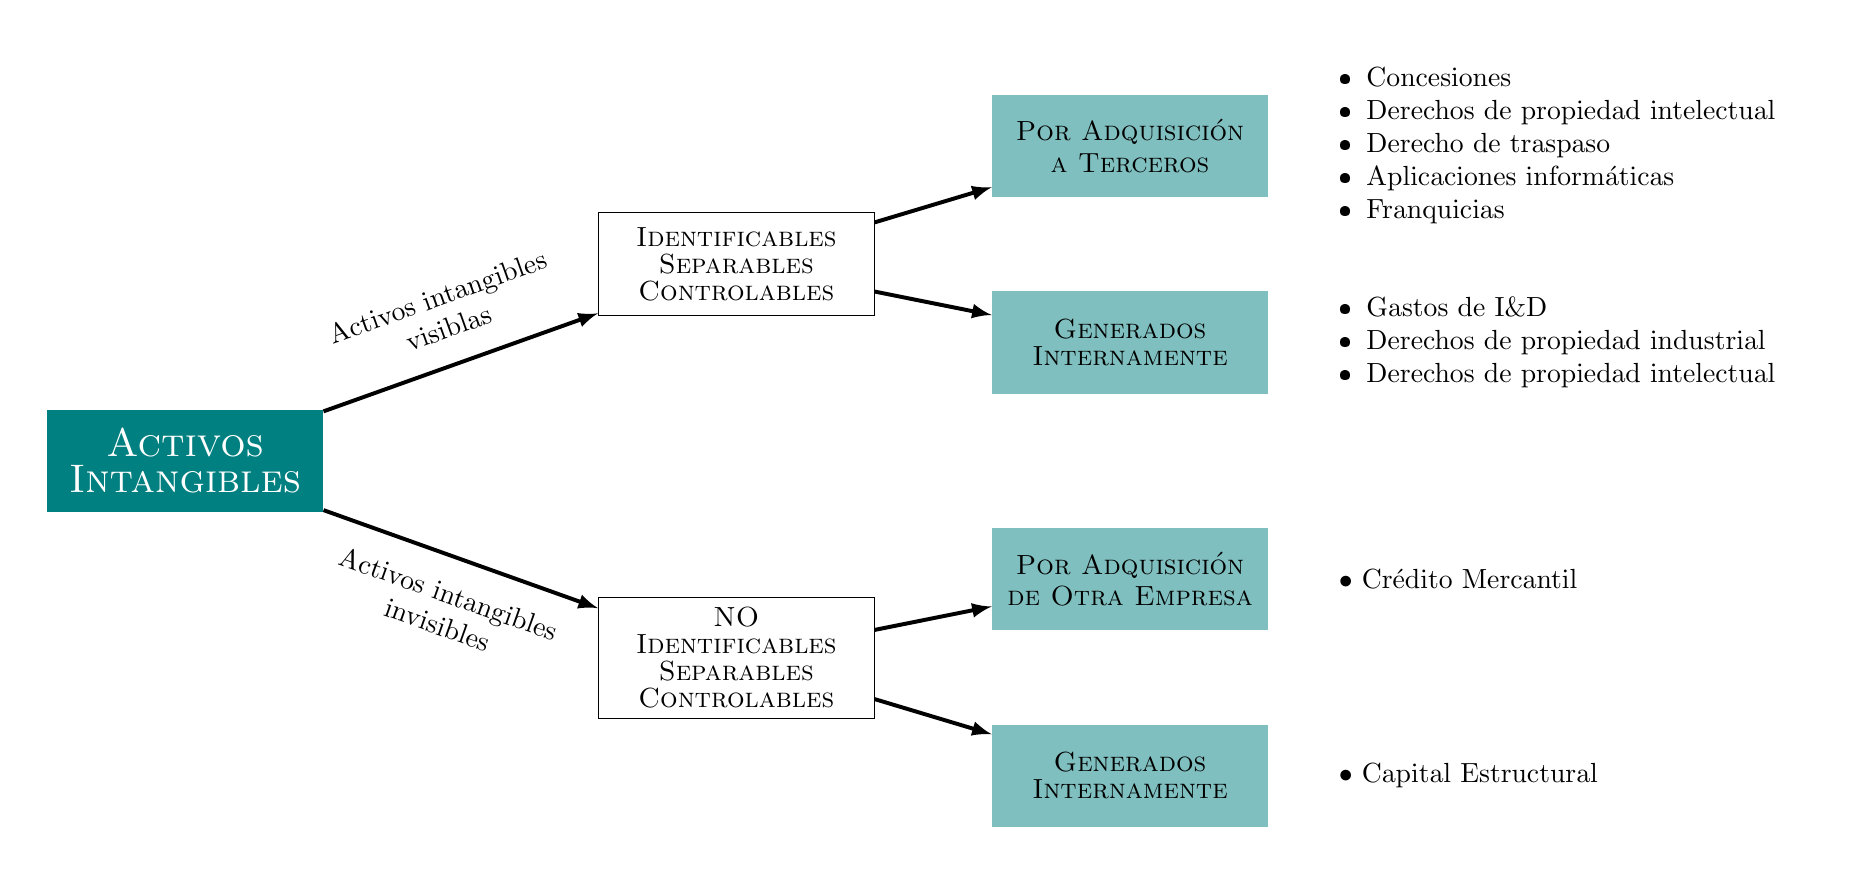
\begin{tikzpicture}[minimum width=3.5cm,minimum height=1.3cm]
	\clip (-4,-5) rectangle (19,5.5);
	\scshape 
	\node [rectangle, fill = teal,text= white] (a) at (-2,0) 
	{\Large \shortstack{Activos \\ Intangibles}};
	\node [draw=black] (b) at (5,2.5) 
	{\shortstack{Identificables \\ Separables \\ Controlables}};
	\node [draw=black] (c) at (5,-2.5) 
	{\shortstack{NO \\ Identificables \\ Separables \\ Controlables}};
	\node [rectangle, fill = teal!50, text=black] (d) at (10,4) 
	{\shortstack{Por Adquisición \\ a Terceros}};
	\node [rectangle, fill = teal!50, text=black] (e) at (10,1.5) 
	{\shortstack{Generados \\ Internamente}};
	\node [rectangle, fill = teal!50, text=black] (f) at (10,-1.5) 
	{\shortstack{Por Adquisición \\ de Otra Empresa}};
	\node [rectangle, fill = teal!50, text=black] (g) at (10,-4) 
	{\shortstack{Generados \\ Internamente}};
	\normalfont
	\node [right] at (12,4) {\vbox{
		\begin{itemize}[noitemsep]
			\item Concesiones
			\item Derechos de propiedad intelectual
			\item Derecho de traspaso
			\item Aplicaciones informáticas
			\item Franquicias
		\end{itemize}
	}};
	\node [right] at (12,1.5) {\vbox{
		\begin{itemize}[noitemsep]
			\item Gastos de I\&D 
			\item Derechos de propiedad industrial 
			\item Derechos de propiedad intelectual
		\end{itemize}
	}};
	\node [right] at (12,-1.5) {\vbox{\(\bullet\) Crédito Mercantil}};
	\node [right] at (12,-4) {\vbox{\(\bullet\) Capital Estructural}};
	\begin{scope}[line width=0.5mm, -latex]
		\draw (a) to node[above ,sloped] 
		{\shortstack{Activos intangibles \\ visiblas}} (b);
		\draw (a) to node[below,sloped] 
		{\shortstack{Activos intangibles \\ invisibles}} (c);
		\draw (b) -- (d);
		\draw (b) -- (e);
		\draw (c) -- (f);
		\draw (c) -- (g);
	\end{scope}
\end{tikzpicture}

\end{document}
